\documentclass[letterpaper, 12pt]{article}
\usepackage[margin=1in]{geometry}
\usepackage{multicol}
\usepackage{paracol}
\usepackage{graphicx}
\graphicspath{{Figures/}{./}}
\usepackage{apacite}
\usepackage{amsmath}
% \usepackage{derivative}
\usepackage{amssymb}
\usepackage{amsthm}
\usepackage{indentfirst}
\usepackage{siunitx}
\usepackage[justification=centering]{caption}
\usepackage{float}
\usepackage{url}

\pagenumbering{roman}

\title{PHYSICS SL
\\
Barton's Pendulum}
\author{}
\date{}

\begin{document}
\nocite{*}

\maketitle
\begin{center}
    Candidate Code:
    \\
    Session: May 2024
    \\
    Page Count:
\end{center}
\newpage

\tableofcontents
\newpage

\pagenumbering{arabic}
\setcounter{page}{1}

\section{Research Question}

What is the relationship between the amplitude of
the forced pendulum /\unit{rad} and the
angular frequency of the driver pendulum /\unit{rad.s^{-1}} in a Barton's pendulum.

\section{Introduction}

Pendulums undergo a repeating cycle of energy transfer from
only potential energy to only kinetic energy back to
only potential energy. This process causes
a pendulum system to undergo simple harmonic motion,
therefore pendulums have properties such as
period and frequency of oscillation defined
that are dependent on the length of the pendulum.

What this also means is that any periodic
external force will or will not resonate with
the pendulum. This applies to various real-life
scenarios and problems, from something as little
as the frequency that a parent should push
their child on a swing to whether gusts
of wind are capable of driving an idle wrecking ball
to dangerous.

Intuitively, if an external periodic force
is resonant with the pendulum, then the extent
that the pendulum's amplitude will reach
will be at its maximum. However, one should question exactly
how this maximum amplitude grows as the frequency
of the external force approaches the resonant frequency
of the pendulum.

This could easily be investigated by suspending
a driving pendulum and a forced pendulum on
the same string. This allows for an easy way
to provide an external periodic force through
the driver pendulum, allowing for the frequency
of the external force to be manipulated through
changing the length of the driver pendulum and
removing the necessity of a motorized
instrument.

\section{Background information} \label{sec:bgInfo}

\subsection{Friction in a pendulum}

Because a pendulum is not sliding along a surface,
then friction cannot be defined by the formula
\(F_f = \mu F_N = \mu_d R\). However, a pendulum
behaves alike to a particle experiencing frictional force
that is proportional to its velocity \cite{FrictionalForceProportional2021}.
It can therefore be defined as

\begin{equation} \label{eq:frictionVelocity}
    F_f = -\gamma v
\end{equation}
\[
    \text{Where } \gamma = \text{the coefficient of friction of an object experiencing friction through drag}
\]

Note that the negative sign is necessary, as the direction
of translational velocity of the pendulum
opposes the direction of frictional force.

\begin{figure}[H]
    \centering
    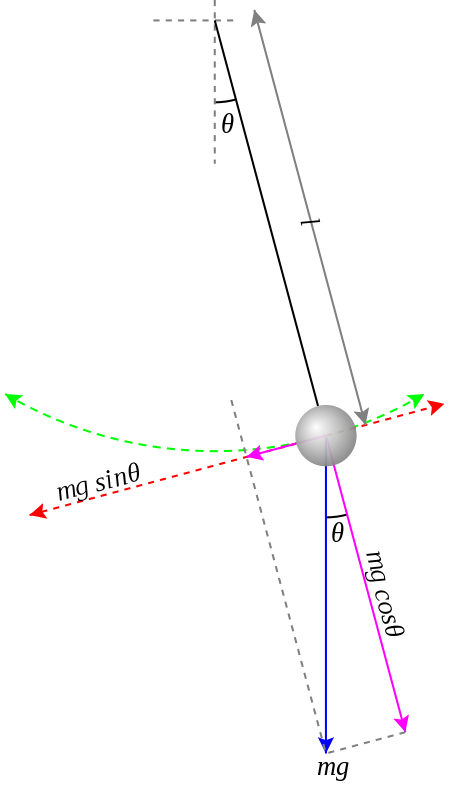
\includegraphics[width=0.5\textwidth]{labelledPendulum.png}
    \caption{Pendulum labelled with components of gravitational force \protect\cite{krishnavedalaEnglishDiagramDepicting2013}.}
    \label{fig:labelledPendulum}
\end{figure}

With reference to Figure \ref*{fig:labelledPendulum}, the
displacement along the green arc (\(s\)) can be defined
below using the definition of a radian.

\begin{equation} \label{eq:defineS}
    s = l\theta
\end{equation}
\[
    \text{Where } l = \text{the length of the forced pendulum } /\unit{m}
\]

Differentiating both sides of Equation \ref*{eq:defineS},
the following relationship is obtained.

\begin{equation}
    \dot s = v = l \dot \theta
\end{equation}

This means that Equation \ref*{eq:frictionVelocity} can be rewritten as
\begin{equation}
    F_f = -\gamma l \dot\theta
\end{equation}

\subsection{External periodic force on a pendulum}

The external periodic force on a pendulum can be modelled as follows

\begin{equation}
    F_e = A_e \cos (\Omega t)
\end{equation}

\begin{align*}
    \text{Where } F_e & = \text{the external periodic force acting on the pendulum } /\unit{N}
    \\
    A_e               & = \text{the amplitude of the external periodic force } /\unit{N}
    \\
    \Omega            & = \text{the angular frequency of the external periodic force } /\unit{rad.s^{-1}}
    \\
    t                 & = \text{duration of time passed after a reference moment in time } /\unit{s}
\end{align*}

\subsection{The Damped, Driven Pendulum}

In Figure \ref*{fig:labelledPendulum}, the component of
gravitational force parallel to the instantaneous velocity of
the pendulum is \(mg\sin\theta\). However, when letting
\(F_g\) equal to such component of gravitational force,
it must equal to the negative of \(mg\sin\theta\)
such that the directionality of \(F_g\) opposes
the directionality of the horizontal component
of \(s\).

\begin{equation}
    F_g = -mg\sin\theta
\end{equation}

\begin{figure}[H]
    \centering
    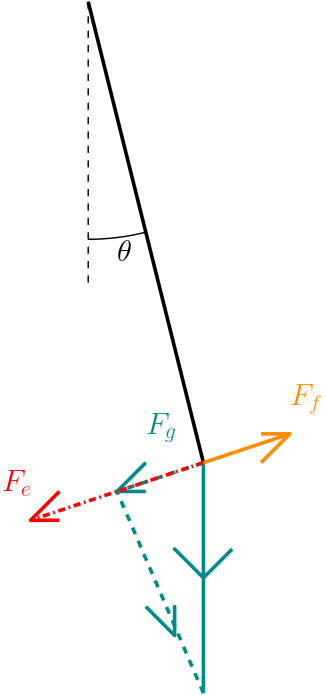
\includegraphics[width=0.2\textwidth]{forcesOnPendulum.png}
    \caption{A pendulum with relevant forces labelled}
    \label{fig:f_netPendulum}
\end{figure}

With reference to Figure \ref*{fig:f_netPendulum}, Equation \ref*{eq:noApproximate}
can be derived as follows.

\begin{align*}
    F_{net}                                                                & = ma
    \\
    F_g + F_f + F_e                                                        & = ma
    \\
    -mg\sin\theta - \gamma l\dot\theta + A_e \cos (\Omega t)               & = m\ddot s \tag{A} \label{eq:simpleNewton}
    \\
    \\
    m\ddot s                                                               & = -mg \sin\theta
    \\
    l\ddot \theta                                                          & = -g\sin\theta \tag{B} \label{eq:gsin}
    \\
    \ddot\theta                                                            & = -\frac{g}{l}\sin\theta
    \\
    \because \omega                                                        & = \sqrt{\frac{g}{l}}
    \\
    \ddot\theta                                                            & = -\omega^2\sin\theta \tag{C} \label{eq:angAccel_Vel}
    \\
    \\
    \text{Substituting \ref*{eq:gsin} into \ref*{eq:simpleNewton}}         &
    \\
    ml\ddot\theta - \gamma l\dot\theta + A_e \cos (\Omega t)               & = m\ddot s \tag{D} \label{gsinSubstituted}
    \\
    \text{Substituting \ref*{eq:angAccel_Vel} into \ref*{gsinSubstituted}} &
    \\
    -ml\omega^2\sin\theta - \gamma l\dot\theta + A_e \cos (\Omega t)       & = m\ddot s
    \\
    \because \ddot s                                                       & = l\ddot \theta
    \\
    A_e\cos(\Omega t)                                                      & = ml\ddot \theta + \gamma l\dot\theta + ml\omega^2\sin\theta
    \\
    \text{Letting } C                                                      & = \frac{A_e}{ml}
    \\
    \lambda                                                                & = \frac{\gamma}{m}
\end{align*}
\begin{equation} \label{eq:noApproximate}
    \ddot\theta + \lambda\dot\theta + \omega^2\sin\theta = C\cos(\Omega t)
\end{equation}

A formula to determine the amplitude of a damped, driven pendulum
can be then determined.

\begingroup
\allowdisplaybreaks
\begin{align*}
    \text{Using the small}                           & \text{ angle approximation of }    \sin\theta \approx \theta
    \\
    \ddot\theta + \lambda\dot\theta + \omega^2\theta & = C\cos(\Omega t)
    \\
    \ddot z + \lambda\dot z + \omega^2 z             & = Ce^{i\Omega t}
    \\
    \text{The ansatz for }                           & z \text{ is } Ae^{i\Omega t} ~\text{\cite{chasnov11DampedDriven2022}}
    \\
    \dot z = i\Omega Ae^{i\Omega t},                 & \quad \ddot z = -\Omega^2 Ae^{i\Omega t}
    \\
    -\Omega^2 A + i\lambda\Omega A + \omega^2 A      & = C
    \\
    A                                                & = \frac{C}{(\omega^2 - \Omega^2) + i\lambda\Omega} \times \frac{(\omega^2 - \Omega^2) - i\lambda\Omega}{(\omega^2 - \Omega^2) - i\lambda\Omega}
    \\
    A                                                & = \frac{C\left[ (\omega^2 - \Omega^2) - i\lambda\Omega \right]}{(\omega^2 - \Omega^2)^2 + \lambda^2\Omega^2}
    \\
    \text{Using the exponential}                     & \text{ form of complex numbers: } a + bi = re^{i\phi}
    \\
    (\omega^2 - \Omega^2) - i\lambda\Omega           & = e^{i\phi} \sqrt{(\omega^2 - \Omega^2)^2 + \lambda^2\Omega^2}
    \\
    A                                                & = \frac{Ce^{i\phi}}{\sqrt{(\omega^2 - \Omega^2)^2 + \lambda^2\Omega^2}}
    \\
    \theta (t)                                       & = \Re (Ae^{i\Omega t})
    \\
    \theta (t)                                       & = \Re (e^{i\Omega t} \frac{Ce^{i\phi}}{\sqrt{(\omega^2 - \Omega^2)^2 + \lambda^2\Omega^2}})
    \\
    \theta (t)                                       & = \Re (e^{i(\Omega t + \phi)}) \frac{C}{\sqrt{(\omega^2 - \Omega^2)^2 + \lambda^2\Omega^2}}
    \\
    \theta (t)                                       & = \left(\frac{C}{\sqrt{(\omega^2 - \Omega^2)^2 + \lambda^2\Omega^2}}\right) \cos(\Omega t + \phi)
\end{align*}
\endgroup

\begin{equation} \label{eq:unlinearized}
    A = \frac{C}{\sqrt{(\omega^2 - \Omega^2)^2 + \lambda^2\Omega^2}}
\end{equation}

Equation \ref*{eq:unlinearized} assumes that:
\begin{itemize}
    \item Due to the small angle approximation made, \(\theta\) does not exceed \(13.99^{\circ}\)
\end{itemize}

All derivations and ideas within Section \ref*{sec:bgInfo} were with reference to \cite{chasnov11DampedDriven2022}.

\section{Hypothesis}

When the length of the driver pendulum equals to the length of the forced pendulum,
then the amplitude of the forced pendulum will be at its maximum as the two pendulums
are in resonance.

As the length of the driver pendulum approaches the length of the forced pendulum,
then the amplitude of the forced pendulum will approach that maximum from lower values.
\\

A more detailed hypothesis can be made by referring to and modifying Equation \ref*{eq:unlinearized}.
\begin{align*}
    A             & = \frac{C}{\sqrt{(\omega^2 - \Omega^2)^2 + \lambda^2\Omega^2}}
    \\
    A^2           & = \frac{C^2}{(\omega^2 - \Omega^2)^2 + \lambda^2\Omega^2}
    \\
    A^2           & = \frac{C^2}{\Omega^4 + (\lambda^2 - 2\omega^2)\Omega^2 + \omega^4}
    \\
    \frac{1}{A^2} & = \frac{\Omega^4 + (\lambda^2 - 2\omega^2)\Omega^2 + \omega^4}{C^2}
\end{align*}

\begin{equation} \label{eq:modified}
    \frac{1}{A^2} = \frac{1}{C^2}\Omega^4 + \frac{\lambda - 2\omega^2}{C^2}\Omega^2 + \frac{\omega^4}{C^2}
\end{equation}

Unfortunately, Equation \ref*{eq:modified} cannot be manipulated further
to achieve a linearized form. However, that doesn't remove
the possibility of analysis despite its form.

If \(\frac{1}{A^2}\) is graphed as a function of \(\Omega^2\),
a parabola opening upwards should be expected as
none of the variables in
\(C = \frac{A_e}{ml}\) can be negative. Additionally,
the question of in which quadrant does the vertex lay can
be answered by taking the derivative of Equation \ref*{eq:modified}
with respect to \(o = \Omega^2\) and solving for \(o\) when
the derivative equals to 0.

\begin{align*}
    \frac{1}{A^2}                                           & = \frac{1}{C^2}o^2+ \frac{\lambda - 2\omega^2}{C^2}o + \frac{\omega^4}{C^2}
    \\
    \frac{\partial}{\partial o}\left( \frac{1}{A^2} \right) & = \frac{2}{C^2}o + \frac{\lambda - 2\omega^2}{C^2} = 0
    \\
    o = \Omega^2                                            & = \omega^2 - \frac{\lambda}{2}
\end{align*}

With reference to Equation \ref*{eq:frictionVelocity} that states
\(F_f = -\gamma v\), it may be assumed that \(F_f \ll v\),
therefore causing \(\lambda = \frac{\gamma}{m}\) to be
insignificant. Because both \(\omega\) and \(A\) can only
be positive given their contexts, the vertex of
\(\frac{1}{A^2}\) as a function of \(\Omega^2\)
must be in the first quadrant.

The specific relationship of \(A\) as a function of \(\Omega\)
can be viewed by graphing such a function through
Equation \ref*{eq:modified}. This is shown in Figure
\ref*{fig:hypothesis}, which the shape of the curve
makes sense given that there is a maximum
at the resonant angular frequency.

\begin{figure}[H]
    \centering
    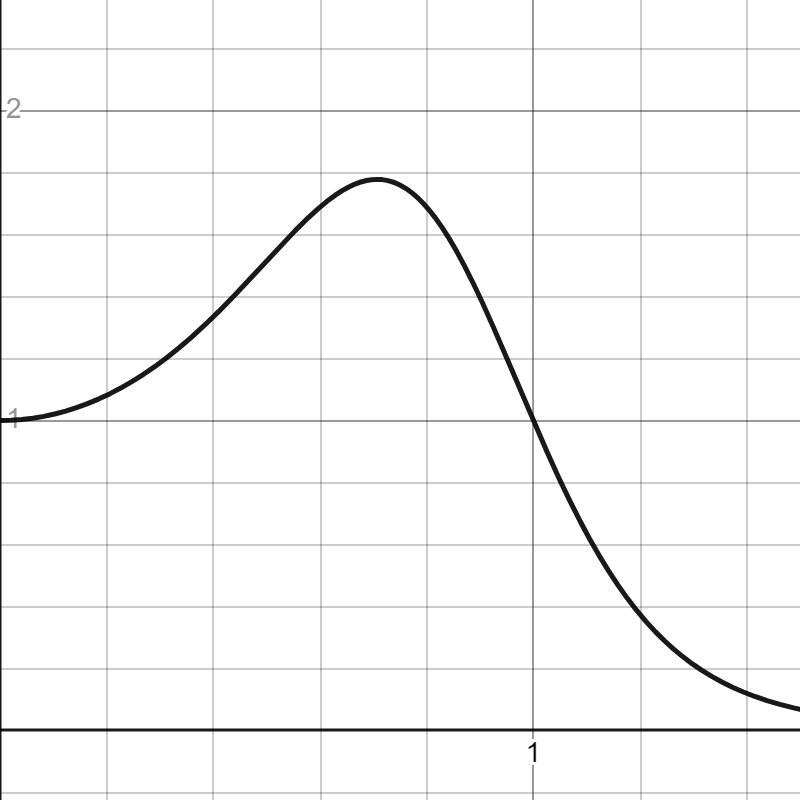
\includegraphics[width=0.5\textwidth]{hypothesis.png}
    \caption{Amplitude of forced pendulum as a function of angular frequency of the driver pendulum graph using Desmos to present a hypothesis of the function's curve shape}
    \label{fig:hypothesis}
\end{figure}

\section{Materials}

\begin{multicols}{2}
    \begin{itemize}
        \item (3) Retort Stands
        \item (2) C-clamps
        \item (4) Clamps
        \item (2) Rulers
        \item (2) Meter Sticks
        \item (1) \SI{200}{g} weight
        \item (1) \SI{50}{g} weight
        \item Tape
        \item String
        \item Paper
        \item Scissors
        \item Highlighter
        \item Phone Camera
    \end{itemize}
\end{multicols}

\section{Variables}

\subsection{Manipulated Variable}
The manipulated variable is the angular frequency of the driver pendulum
/\unit{rad.s^{-1}}. In this lab, the manipulated variable will be changed
by shortening the length of the string. This change will be measured by
PASCO Capstone's distance measurement tool.

\subsection{Responding Variable}
The responding variable is the amplitude of the forced pendulum /\unit{rad}.
The responding variable will be measured using PASCO Capstone's
object tracking tool.

\subsection{Controlled Variables}

The first controlled variable will be the starting amplitude of the
driver pendulum. This variable will be controlled by setting up a
meter stick with its foot pivoted on a retort stand at a
consistent position while leaning on the meter stick
sitting on top of the clamps between the two primary retort
stands, where each trial involved pushing the driver pendulum up to the
angle of that leaning meter stick. This variable must be controlled in
order to ensure that any changes in the amplitude of the forced
pendulum between trials isn't a result of varying
initial amplitude of the
driver pendulum and therefore inconsistent total energy in the system.
This controlled variable is also seen in Equation \ref*{eq:unlinearized}
from \(C = \frac{A_e}{ml}\), where \(A_e\) is the
amplitude of the external periodic force.

The second controlled variable will be the tension in the
master string that both pendulums are suspended from. This variable
will be controlled by using the same string of a consistent length
and maintaining the positions of the primary retort
stands with C-clamps. This variable must be controlled to
ensure that the degree of energy exchange between the
two pendulums is consistent between trials. Additionally,
overly loose strings will cause the degree of oscillation
in the master string to drastically effect the data.

The third controlled variable is the length of the
forced pendulum. This variable will be controlled by not
exchanging the string of the forced pendulum between trials.
This variable must be controlled to ensure that the
angular frequency of the forced pendulum seen
in Equation \ref*{eq:unlinearized} as \(\omega\)
remains consistent. It also ensures that \(C\)
remains consistent as \(C = \frac{A_e}{ml}\),
where \(l\) is the length of the forced pendulum.

The fourth controlled variable is the mass of
the forced pendulum. This variable will be controlled by
avoiding the exchange of weights of different
masses for the forced pendulum between trials.
This variable must be controlled to
ensure that the parameters of \(C = \frac{A_e}{ml}\)
and \(\lambda = \frac{\gamma}{m}\) remain consistent.

\section{Experimental Protocol}

\section{Raw Data}

\section{Processed Data}

\section{Analysis}

\section{Evaluation}

\bibliographystyle{apacite}
\bibliography{IB_PHYSICS_IA.bib}

\end{document}